\section{Problem and Experimental Setting}
\label{sec:setting}

\paragraph{Scenes, edits and groups.}
A scene contains three objects, each with a shape (cube, sphere, cylinder, cone), a colour (red,
blue, green, yellow, purple), a material (metal, rubber) and one of three horizontal slots; no two
objects are identical. Four edit operations act on scenes: a \emph{binding} edit swaps one
attribute type between two objects; an \emph{attribute} edit replaces one attribute value; an
\emph{object} edit replaces one shape; and a \emph{relation} edit swaps the slots of two objects.
Each operation carries an explicit contract on scene metadata. For example, a binding edit must
leave the multisets of shapes, colours and materials unchanged while changing the multiset of
(shape, attribute) pairs. Edits that violate their contract, such as swapping colours between two
cubes, are rejected. A caption lists every object in one of three templates (for example
``a red metal cube'' or ``a cube that is red and metal'') and adds one relation clause
(``the X is left of the Y''). Object order, template and relation direction vary between captions
and are independent of the scene layout. A \emph{group} consists of a base scene, an edited scene
and their captions under the same paraphrase choice, with member order randomized. An oracle
decides whether a caption is true of a scene by searching for an injective assignment of described
objects to scene objects. A group is kept only if its $2{\times}2$ truth table is the identity:
each caption is true for its own scene and false for the other.

\paragraph{Two input conditions.}
The first version of this setting (v0) fed the model one token per object, computed as the sum of
fixed embeddings of that object's shape, colour, material and slot. These tokens are a function of
the scene graph and already bind each object's attributes, so any binding result obtained with
them is a statement about the text side and the alignment, not about visual binding. We therefore
treat them only as an \emph{oracle object-token control}. In the pixel condition (v1), a minimal
renderer draws each scene as a $224{\times}224$ RGB image (Figure~\ref{fig:examples}). Shapes are
drawn with distinct silhouettes and faces, colours from a fixed palette with shading, metal with
high-contrast shading and a specular highlight, and rubber with matte shading. Each slot is a
horizontal column, so ``left of'' in the scene graph is exactly the $x$-order in the image. Each
render seed adds position and size jitter, a background level and pixel noise. Images are encoded
by a frozen OpenCLIP ViT-B/32 model trained on LAION-2B \citep{ilharco2021openclip,
schuhmann2022laion5b}, pinned by revision and checksum. The model inputs are the final-layer class
token and 49 patch tokens, each projected to the 512-dimensional joint space. Captions are encoded
as raw strings into per-token states from the start to the end token. Scene metadata is used only
by the renderer, the oracle labels and the training masks; the encoder interface accepts only
images and strings, and a test checks that no model scorer reads metadata.

\begin{figure}[t]
\centering
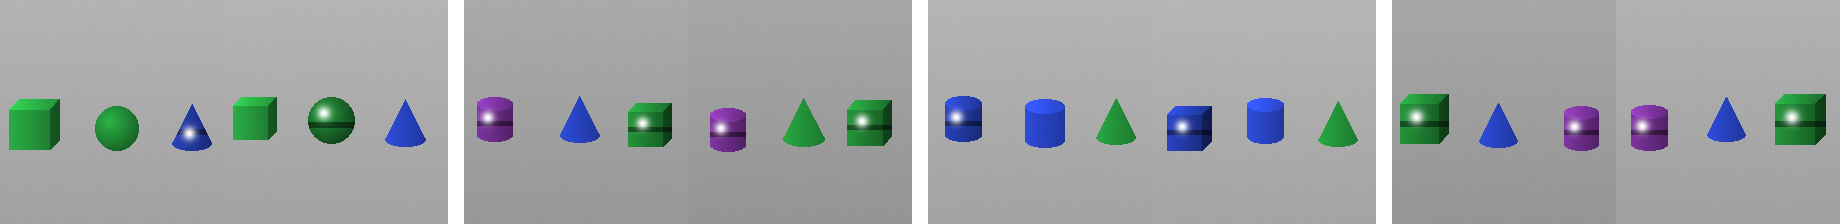
\includegraphics[width=\linewidth]{figures/dev_examples_row.png}
\caption{The first four development groups in generation order (not selected by model
performance). Each pair shows the two members of one group. The pixels are those of the run output
\texttt{dev\_examples.png}, re-tiled into one row by \texttt{scripts/make\_paper\_figures.py}.}
\label{fig:examples}
\end{figure}

\paragraph{Edit orbits and splits.}
Binding and relation edits generate a group action on scenes: transpositions of colours, of
materials or of slots between objects generate all permutations of each attribute type, with shapes
attached to object identities. Ignoring the validity constraint on intermediate scenes, the
\emph{edit orbit} of a scene under this action is the set of valid scenes with the same multisets
of shapes, colours and materials (positions always fill the three slots), and the split key is
exactly this triple of multisets. Attribute and object edits change these multisets and so move a scene to a
different orbit. Data v0 prevented leakage at the level of scenes and caption contents, so all
render variants and paraphrases of a scene or caption stayed in one split. Data v1 adds the orbit
as a leakage unit: every orbit is assigned to one split by a hash of its key, base scenes are drawn
only from the split's orbits, and an edit is kept only if its result stays in an orbit owned by the
same split. This restriction changes the distribution of accepted content edits relative to
unrestricted sampling; Appendix~\ref{app:splits} reports the measured proposal and acceptance
counts instead of assuming uniformity. Data v1 uses a fresh seed and the v0 split sizes
(\DVnTrain{} training, \DVnDev{} development, \DVnCalib{} calibration and \DVnTestIid{},
\DVnTestHeldoutPairs{}, \DVnTestComposition{} and \DVnTestHeldoutTemplate{} groups in the four test
splits). The v0 test splits were scored during an early technical smoke run and are treated as
development material; no model has been scored on any v1 test split.

\paragraph{Binding-necessary endpoint.}
A group is \emph{binding-necessary} (\bn) when all of its edits are binding or relation edits.
Equivalently, both of its scenes lie in the same orbit, so the two images contain the same objects
and attribute values and differ only in their assignment or arrangement. The subset is defined by
metadata alone and never by model scores. It is the primary endpoint because on groups with content
edits a binding-blind signal can succeed: in the v0 smoke run (oracle tokens, first 100 groups of
the v0 composition split), the content-only channel of each trained head reached GroupMatch
\SMcontentMatchMin--\SMcontentMatchMax{}, against a chance level of $0.5$.

\paragraph{Head and scorer.}
The trainable head is shared by all conditions. For a set of image tokens $\{v_k\}_{k=1}^{n}$ it
outputs a content part $c = W_c\,\tfrac1n\sum_k v_k$ and a binding part
$b = \tfrac1n\sum_k (A v_k)\odot(A' v_k)$. For text tokens $\{u_t\}_{t=1}^{L}$ the binding part is
$\tfrac1L\sum_t\sum_{\delta\in\pm\{1..5\}}\alpha_\delta (B u_t)\odot(B' u_{t+\delta})$ with learned
offset weights $\alpha_\delta$. The score is the inner product
$s(I,T)=\langle [c_I;b_I],[c_T;b_T]\rangle$. With 8 content and 8 binding dimensions and
512-dimensional inputs, the head has \SPheadParams{} parameters; the frozen encoder has
\SPencParams. Tokens are standardized per dimension with statistics of the training panel.
With the additive oracle tokens of v0, the content part is exactly invariant to binding and relation
edits by construction. With CLIP tokens this invariance no longer holds, and we measure it instead
of assuming it (Section~\ref{sec:experiments}).

\paragraph{Metrics, ties and chance levels.}
For a group with score matrix $S_{ij}=s(I_i,T_j)$, the Winoground \emph{text} score requires
$S_{00}>S_{01}$ and $S_{11}>S_{10}$, the \emph{image} score requires $S_{00}>S_{10}$ and
$S_{11}>S_{01}$, and the \emph{group} score requires both \citep{thrush2022winoground}.
\emph{GroupMatch} requires $S_{00}+S_{11}>S_{01}+S_{10}$ \citep{zhu2025ttm}. With a meaning-preserving
paraphrase $T'_i$ of each caption, \emph{aug} counts images for which both $T_i$ and $T'_i$ beat
$T_{1-i}$, and \emph{aug\_group} requires this for both images \citep[after][]{kamath2024hardpositive}.
The \emph{pair AUC} treats the four image--caption pairs of each group as a binary ranking problem
labelled by the oracle. All comparisons are strict with a relative tolerance of $10^{-9}$, so ties,
including round-off differences between mathematically equal scores, count as failures. AUC
assigns tied scores their average rank. For independent continuous scores the chance levels are
$1/4$ (text, image), $1/6$ (group), $1/2$ (GroupMatch), $1/3$ (aug), $1/9$ (aug\_group) and $0.5$
(pair AUC). Each is derived separately in Appendix~\ref{app:chance}; we do not transfer the $1/k!$
formula for GroupMatch to other metrics. A Monte-Carlo check on the development panel gives
\SPchanceGroupMC{} for group and \SPchanceMatchMC{} for GroupMatch.

\paragraph{Controls.}
We report an oracle scorer (metadata truth, an upper bound for the evaluation code), zero-shot CLIP
cosine scores, a text-only n-gram logistic regression and an image-only logistic regression on
pooled CLIP features, the content-only and binding-only channels of the trained head, the trained
head with development images or captions shuffled across groups, and the same head trained on
oracle object tokens. On $2{\times}2$ groups a single-modality scorer produces two identical rows or
columns. Every comparison therefore ties, and its text, image, group and GroupMatch scores are zero
by construction. Its pair AUC is exactly $0.5$ because every caption, and every image, appears once
with each label (Appendix~\ref{app:blind}). These values are properties of the design, not evidence
that the benchmark is free of artefacts. For artefacts, the informative checks are the content-only
channel, the shuffles, and classifiers that try to tell base from edited scenes.
